\documentclass{mprop}
\usepackage{graphicx}
\usepackage{algorithm}
\usepackage{algpseudocode}
\usepackage{float}
\usepackage{siunitx}
\usepackage{xspace}
\usepackage{cite}
\usepackage{pgfgantt}

\graphicspath{ {images/} }

% alternative font if you prefer
% \usepackage{times}

% for alternative page numbering use the following package
% and see documentation for commands
\usepackage{fancyheadings}


% other potentially useful packages
\usepackage{amssymb,amsmath}
%\usepackage{url}
%\usepackage{fancyvrb}
%\usepackage[final]{pdfpages}

\begin{document}

%%%%%%%%%%%%%%%%%%%%%%%%%%%%%%%%%%%%%%%%%%%%%%%%%%%%%%%%%%%%%%%%%%%
\title{Probabilistic Topic Modelling for Spatial Smoothing in Mass Spectrometry Imaging}
\author{Arijus Pleska}
\date{Date of submission placed here}
\maketitle
%%%%%%%%%%%%%%%%%%%%%%%%%%%%%%%%%%%%%%%%%%%%%%%%%%%%%%%%%%%%%%%%%%%

%%%%%%%%%%%%%%%%%%%%%%%%%%%%%%%%%%%%%%%%%%%%%%%%%%%%%%%%%%%%%%%%%%%
\tableofcontents
\newpage
%%%%%%%%%%%%%%%%%%%%%%%%%%%%%%%%%%%%%%%%%%%%%%%%%%%%%%%%%%%%%%%%%%%

%%%%%%%%%%%%%%%%%%%%%%%%%%%%%%%%%%%%%%%%%%%%%%%%%%%%%%%%%%%%%%%%%%%

% Metabolomics
% Mass Spectrometry
% Vision
\section{Introduction}

% To-do:
% - Ionisation
% - Mass Spectrum

% Notes:
% -- Mass spectrum measures the masses of the ions entering mass spectrometer. For this reason, the sample has to be ionised beforehand.
% -- The ionisation process takes the molecules of a metabolite and a adds to something like a `proton'. Then, the resulting measure of mass would be the metabolite plus the proton.


% Structure:
% 1. General statement of the proposal (novel techniques for the analysis in Mass Spectrometry Imaging (MSI))
% 2. Mass Spectrometry Imaging. What is it used for?
% 3. Challenges in the analysis of MSI data.
% 4. Your contributions to the domain.
% 5. Report outline.


% Intro
% - ML in biology
% - MSI
% - Spatial Smoothing
\par This proposal is focused on applying machine learning techniques to improve the analysis of biology data sets. We intend to enhance the quality of \textit{mass spectrometry imaging} (MSI) data. Briefly, by the use of MSI, the researchers are able to interpret the formation of chemical processes. However, as suggested by a recent overview by Smith et al. \cite{smith_2004}, the pre-processing of molecular-level entity data sets is lagging in terms of the current noise reduction algorithm effectiveness. We will attempt to tackle this issue of noise by utilising spatial smoothing. 
  

% MSI
% - Connection to metabolomics
% -- Metabolomics definition
% - Vision
% - Chemical Process occurrence

\par In this project, the application domain of MSI is set to be \textit{metabolomics} -- it is the scientific study of chemical processes which involve metabolites (small molecules) and metabolomes (sets of small molecules). In the settings of metabolomics, we utilise \text{mass spectrometry} (MS) to obtain the distribution of chemical entities within a sample. By utilising MSI, we can visualise the distributions of the ions (or ion sets) of different masses. For instance, Figure \ref{fig:b_and_e} below represents a captured sample as an image, where each picture's pixel is a small region within the sample. 
\begin{figure}[H]
  \centering
  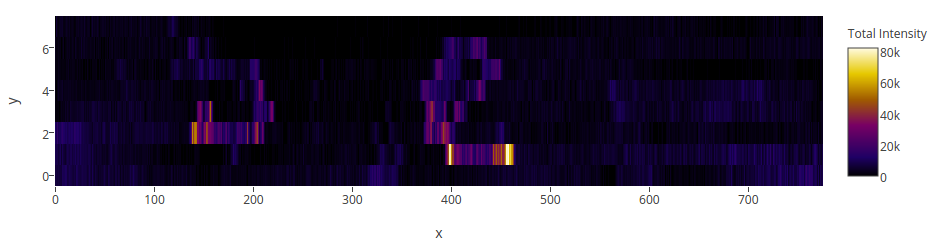
\includegraphics[width=0.7\textwidth]{b_and_e}
  \caption{MSI application on a sample with the letters b and e.}
  \label{fig:b_and_e}
\end{figure}
Note that each pixel contains a distribution of chemical entities as well. In Figure \ref{fig:b_and_e} we have chosen the range of mass to reflect the ink used to inscribe the letters. That is, in each pixel we have summed the intensities of the chemical entities meeting the mass criteria. Then, each pixel has been assigned an intensity value. Therefore, the sample could be expressed as the latter image. An open problem in metabolomics is to find the sets of chemical entities  inducing valid visual patterns. Ultimately, the discovered biological patterns could be used to suggest and measure the likelihood of a particular chemical process occurrence. For a rigorous discussion on machine learning applications in metabolomics, the reader can consult the recent survey conducted by Alonso et al. \cite{alonso-et-al}.

% -- The ionisation process might be executed in different means. This results in a different sum of masses.
% -- Metabolite might be fragmentised during the ionisation.
% -- Atoms of the same thing might have a different mass. This would result in the different ion mass.

% Challenges
% - Explanation of the data capturing process
% - Ionisation
% -- Fragmentation
% -- Different means to ionise the metabolite
% -- Atoms might have a different mass
% - Noise
% -- Spatial Smoothing

\par The challenges on working with MSI data arise from the data capturing process. In metabolomics, the MS equipment requires the ionisation of metabolites. Effectively, a metabolite is compounded with an appropriate chemical entity to produce an ion. It follows that the mass spectrometers are capable to capture some properties of the ionised metabolites. Since the mass of an ion belongs to these properties, the collection of captured ions can be represented in terms of mass spectra. However, the following issues have to be considered upon reasoning from the MSI data: (1) the ionisation of a metabolite can be performed using different chemical entities, therefore the ions of same metabolite type would have different masses; (2) a metabolite might be fragmented during the ionisation; (3) the metabolites of same type might have different atom structure, which suggests a different mass value. The latter issues, effectively, corresponds to a problem of error correction.
 
% The domain of vision
% - Expalanation how the scans of metabolites can be treated as images.
% - Visualisation of particular metabolites or metabolite patterns.

% \par In the terms of machine learning applicability, we are looking into a problem of vision. The metabolites of some biological tissue are sequentially captured within regions of fixed size. Effectively, this process is generating an image: each scan is a pixel, therefore, the collections of scans produce an image. However, each pixel contains a large amount of metabolites, so the visualisation of these in a single image would be rather complex. Thereby, we can choose a specific metabolite type and produce pixels reflecting such metabolite activity.  Going back to the visualisation of metabolites, we can choose a specific combination (structure) and produce an image where activated pixels would suggest the concentration of the chosen metabolite structure. The problem arises upon discovering valid matabolite structures. Therefore, the techniques of machine learning, or more specifically topic modelling, are used to induce the prospective structures.

% Unsupervisder learning
% - Topic moels
% - Probabilistic models
% - LDA:
% -- General
% -- Metabolomics
\par Since this proposal is focused on utilising spatial smoothing to reduce the impact of noise in MSI data sets, we will familiarise with the machine learning techniques and problems tackled in the MSI domain. The objective to discover novel patterns can be treated as a problem of \textit{unsupervised} machine learning. That is, we have no initial settings in how the patterns are expected to look like. However, upon appropriate optimisation, the unsupervised machine learning techniques are capable to learn the patterns on their own. To be more specific, we will utilise the techniques of \textit{topic modelling} (in this case, a pattern is referred by a topic). Also, we are focusing on the \textit{probabilistic} (statistical) models, more specifically, \textit{latent Dirichlet allocation} (LDA). First of all, the successor LDA-like models are treated as a state-of-the-art method in tackling semantic-analysis type problems. For more detailed review on the LDA applications, the reader can consult the survey conducted by Blei \cite{blei_2012}. Also, Hooft et al. \cite{hooft} has recently addressed the applicability of LDA in MSI data sets. This proposal is directly influenced by the latter study: we will utilise the LDA-like models to reduce the impact of noise in the MSI data sets.  

% Outline
% - Sections
\par The structure of this proposal is given as follows: in Section 2 we present the issue of noise in MSI data sets; in section 3 we cover the literature in topic modelling which focuses on the variations of LDA-like models; in Section 4 we discuss the approach to tackle the problem (we discuss the reviewed literature, address design and evaluation details); finally, in Section 5, we set and schedule the tasks required to complete the project.
% To-do: rewrite the outline

%%%%%%%%%%%%%%%%%%%%%%%%%%%%%%%%%%%%%%%%%%%%%%%%%%%%%%%%%%%%%%%%%%%%%%%%%
%%%%%%%%%%%%%%%%%%%%%%%%%%%%%%%%%%%%%%%%%%%%%%%%%%%%%%%%%%%%%%%%%%%%%%%%%
%%%%%%%%%%%%%%%%%%%%%%%%%%%%%%%%%%%%%%%%%%%%%%%%%%%%%%%%%%%%%%%%%%%%%%%%%
\section{Statement of Problem}

% Intro
% - Suggesting an advance in processing rather than equipment.
\par Currently, MS equipment is incapable to fully represent the metabolite construction. As discussed by Palmer et al. \cite{palmer},  the current hardware limit in differentiating between the ions in millidalton precision does not mitigate the issue of the false positive data. Thereby, rather than relying upon the advances in MS equipment, we can investigate the prospect of enhancing the data processing techniques. As described in Section 1, LDA derivatives are promising methods in discovering the hidden patterns in MSI data sets. For this reason, we raise a hypothesis that the degeneracies of MSI data sets can be detected using LDA-like models.   

% Objectives
% - Research in the state-of-the-art methodology.
% - Reducing the impact of noise in metabolomics.
% - Providing a general-purpose machine learning model.
\par The primary goal of this research is to expand the consensus on whether topic modelling is a valid approach to apply spatial smoothing in MSI data sets. To be more specific, we set our objectives to the following:
\begin{enumerate}
    \item Optimise the general topic modelling methods for MSI data sets;
    \item Successfully apply spatial smoothing in MSI data sets;
    \item Give a basis to a general topic modelling method for error correction.
\end{enumerate}
Briefly, the first objective is expected to utilise the general state-of-the-art topic modelling methodology to distinguish the techniques displaying better performance in MSI applications -- we will conduct a survey on LDA-like topic modelling methodology. The second objective focuses on optimising those general models for the particular task of spatial smoothing in MSI data sets. Finally, the third objective can be treated as a general contribution to the field of machine learning, since the discovered spatial smoothing techniques might be applicable to other domains. 

% Hypothesis
% - Topic modelling can improve the quality of metabolomics data sets.
% - The negation of the hypothesis would contribute in terms of reassessing the complexity of the problem.
\par The main project hypothesis -- the LDA-like models can detect and correct the degeneracies of MSI data sets -- can be interpreted as the spatial smoothing of MSI data sets. Both cases of proving and disproving this hypothesis would contribute to the research in MSI. The successful outcome would lead to the potential applications discussed in the following paragraph, whereas the unsuccessful outcome would set up additional requirements to tackle the issue of noisiness in MSI data sets.

% Results: tools to annotate the metabolites > basis for generative error correction 
% - Expanding the application of existing machine learning models.
% - Advancing the current state-of-the-art in metabolomics.
% - Contributing to machine learning in general.
\par The potential applications of the successful research outcome can be directly induced from the previously listed objectives. First of all, we would show that the general models (or the models applied in other domains) can be utilised for MSI data analysis. Further, the developed spatial smoothing methodology would improve the accuracy of the chemical processes prediction. Finally, the generalisation of the developed spatial smoothing model might suggest different approaches in tackling error correction in general; finally, the successful research outcome would suggest the applicability prospect of topic modelling in MSI data sets; reversely, it would also impact the prospect to derive machine learning generalisations from the research in MSI data sets.  

%%%%%%%%%%%%%%%%%%%%%%%%%%%%%%%%%%%%%%%%%%%%%%%%%%%%%%%%%%%%%%%%%%%%%%%%%
%%%%%%%%%%%%%%%%%%%%%%%%%%%%%%%%%%%%%%%%%%%%%%%%%%%%%%%%%%%%%%%%%%%%%%%%%
%%%%%%%%%%%%%%%%%%%%%%%%%%%%%%%%%%%%%%%%%%%%%%%%%%%%%%%%%%%%%%%%%%%%%%%%%
\section{Background Survey}

% Intro
% - The reason why the literature review is conducted.
% - Outline: preliminaries, notation, literature.
% - A notification the the results will be discussed in the following section.
\par The provided literature review on topic modelling is directed towards familiarising with LDA derivatives. Also, the review assesses the methodology of LDA-like models and proposes several implementation variations. The review is structured in progressing order: at the start, we look into the original LDA paper and define the terminology (it will be used throughout the proposal); then, we familiarise with two different techniques used for the inference of LDA-like models; finally, we review LDA derivatives which shows the potential to be utilised in designing the error correction technique.

%%%%%%%%%%%%%%%%%%%%%%%%%%%%%%%%%%%%%%%%%%%%%%%%%%%%%%%%%%%%%%%%%%%%%%%%%
%%%%%%%%%%%%%%%%%%%%%%%%%%%%%%%%%%%%%%%%%%%%%%%%%%%%%%%%%%%%%%%%%%%%%%%%%
\subsection{Terminology}

% General intuition on topic modelling
% - Example
\par Recall that in topic modelling induces a hidden structure within the studied data sets. We will provide an example providing an intuition in this process. Say, if we were analysing a book, its chapters might address different topics or address the topics at a different extent. Further, the chapters itself would have unique distributions of the topics. Note that we are assuming that we do not know what the topics addressed in the book. In order to derive these hidden topics, a probabilistic topic modelling method would analyse the structure of the words used in the book. In other words, the model would induce patterns which would refer to a particular topic. Regarding the method's performance, it would depend on the method's ability to optimise the inference of the patterns. For example, commonly used words (such as and, or, the, etc.) would be relevant in all topics. Therefore, their semantic impact in defining the topics would be negligible. For this reason, we could dismiss these to improve the time performance of the method. 

% LDA intro
% - the model
% - A notification that the terminology and the notation will be useful throughout the proposal.
\par The terminology used in this proposal is equivalent to the terminology used by Blei \cite{blei_2012}. Figure \ref{fig:lda} below represents the original LDA model in plate notation. We will use it as a guide to familiarise with the terminology.   
\begin{figure}[H]
  \centering
  \includegraphics[width=0.7\textwidth]{lda_model}
  \caption{The design of the original LDA model}
  \label{fig:lda}
\end{figure}

% High level LDA terminology
% - Notation:
% -- List LDA definitions
% -- Explain the definitions
\par To start with, we will familiarise with the higher level entities of the model. The circles represent an entity, whereas the plates indicate the number of entities. For example, there would $N \times M$ entities of $z$ and $M$ entities of $\theta$. Further, LDA is a three-level hierarchical structure: the smallest entity (grey circle) is defined as a \textit{word}; then a collection of words (inner plate) is defined as a \textit{document}; and a collection of documents (outer plate) is a \textit{corpus}. Note that Figure \ref{fig:lda} represents $M$ documents and $N$ words per document, it follows that in the corpus there would be $M \times N$ words. Also, as suggested by Figure \ref{fig:lda}, let's denote a word by $w$. Then, let's denote the sequence of words in document $d$ by 
\begin{equation*}
\mathbf{w}_d = \{w_1, w_2, \dots, w_N\},
\end{equation*}
then the sequence of words in the corpus would be denoted by
\begin{equation*}
\mathcal{\mathbf{D}} = \{\mathbf{w_1}, \mathbf{w_2}, \dots, \mathbf{w_M}\}.
\end{equation*}
 
% Low level LDA terminology
% - Intro to observable and hidden variables
% - Notation:
% -- List the definitions
% -- Explain the definitions
\par Now, we will introduce the lower level entities. The grey circle indicates that the \textit{observable} variables, whereas the white coloured circles indicate the \textit{hidden} variables. Note that in Figure 1 the words are the only observable variables; all other entities are hidden, i.e., they describe the underlying structure of the model. Further, recall that topic modelling is applied in order to discover a mixture of topics; or in other words, topic modelling could describe a corpus and its documents in terms of topic distributions. This intuition will simplify the definitions of the remaining entities in Figure 1, these are given as follows:
\begin{itemize}
\item $K$ is the number of topics;
\item $V$ is the size of the vocabulary, i.e. the number of unique words in the corpus;
\item $\alpha$ is the parameter referring to the prior distribution of the topics over documents;
\item $\beta$ is the parameter referring to the prior distribution of the vocabulary over topics;
\item $\theta$ is the latent variable referring to the topic distribution over documents;
\item $\phi$ is the latent variable referring to the vocabulary over topics
\item $w$ is the observable variable referring to the words in documents;
\item $z$ is the latent variable of topic assignments over the words.
\end{itemize}
Further, note that the listed entities can be perceived as matrices of the following dimensions: $\alpha$ is $1 \times K$; $\beta$ is $K \times V$; $\theta$ is $M \times K$; $\phi$ is $K \times V$; $w$ is $M \times N$; and $z$ is $M \times V$.
% To-do: check the dimensions

%%%%%%%%%%%%%%%%%%%%%%%%%%%%%%%%%%%%%%%%%%%%%%%%%%%%%%%%%%%%%%%%%%%%%%%%%
%%%%%%%%%%%%%%%%%%%%%%%%%%%%%%%%%%%%%%%%%%%%%%%%%%%%%%%%%%%%%%%%%%%%%%%%%
\subsection{Preliminaries}

% Basic LDA
% - Generative process
% - The derivation of the posterior
\par The relationship the between observable and hidden variables, effectively, describes the inference of the underlying topic structure. We will go through an arbitrary example in order to give an intuition in the inference process and familiarise with the lower level notation of the previous listed variables. Figure \ref{fig:lda} shows see that $\alpha_k$ (the prior for the $k$th topic in a document) influences $\theta_{:, k}$ (the latent variable describing the distribution of topic $k$ over all documents). It follows that $\theta_{d, k}$ (the probability of the $k$th topic occurrence in document $d$) influences $z_{d, :}$ (the topic assignment over all vocabulary terms for document $d$). Further, $z_{d, v}$ refers to the topic assignment of vocabulary term $v$. By taking $z_{d, v}$ and $\beta_{v, k}$ (the prior of topic $k$ on vocabulary term $v$), we obtain word $w_{d, v}$. In the complete perspective, the generative process of the corpus is given by the following joint probability distribution
\begin{equation}
p(\beta, \theta, z, w) = \prod_{k=1}^Kp(\beta_{:, k})\prod_{d=1}^Dp(\theta_{d, :})\bigg(\prod_{v=1}^Vp(z_{d, v} | \theta_{d, :})p(w_{d, v} | \beta, z_{d, v})\bigg).
\end{equation}
By using Bayes Theorem, we derive the computation of the conditional distribution
\begin{equation}
p(\beta, \theta, z | w) = \frac{p(\beta, \theta, z, w)}{p(w)}. 
\end{equation}
This equation expresses the computation of the posterior -- the derivation of the hidden corpus structure given observable variable $w$. The problem arises from inefficient analytical computation of evidence $p(w)$. The approximation of it will be considered during the literature review on LDA-like models. The naming of the following subsections corresponds to the reviewed papers. 

%%%%%%%%%%%%%%%%%%%%%%%%%%%%%%%%%%%%%%%%%%%%%%%%%%%%%%%%%%%%%%%%%%%%%%%%%
%%%%%%%%%%%%%%%%%%%%%%%%%%%%%%%%%%%%%%%%%%%%%%%%%%%%%%%%%%%%%%%%%%%%%%%%%
\subsection{Latent Dirichlet Allocation}

% Intro
% - Detailed approach in covering implementations details
\par Latent Dirichlet allocation is a probabilistic topic modelling technique proposed by Blei et al. \cite{blei_2003}. Since this paper is the origin of LDA-like models, it will be discussed in more detail to introduce the basis of LDA-like methodology. As a result, this coverage will simplify the review on the LDA derivatives discussed in the upcoming subsections. 

% Assumptions 
% - Bag of words principle
% - Discrete data sets
% - Topic dimensionality
\par The original LDA model sets some assumptions for the data processed by the model. First of all, it is assumed that documents and words are \textit{exchangeable}. That is, the order in which these entities are processed does not matter. In other words, we can say the model follows the \textit{bag-of-words} principle. The next assumption states that we should use discrete data. Effectively, the basic LDA does not cover  continuous features. Another assumption is on the number of topics: it is set to be fixed throughout the complete run of inference.  

% Generative process
% - Three level hierarchy
% - The generative algorithm
\par As discussed in the preliminaries subsection, we are also taking an assumption that the corpus is induced by a probabilistic process. The generation of the corpus has three levels: the parameters $\alpha$ and $\beta$ are sampled once; the variable $\theta$ is sampled once per document; and the variables $z$ and $w$ are sampled once per word. This hierarchical process relates to the generative algorithm given in the original LDA paper, it is equivalent to Algorithm 1 below.
\begin{algorithm}[H]
\caption{Document Generation}
\label{alg:document_generation}
\begin{algorithmic}[1]
\State $N \sim \mbox{Poisson}(\xi)$
\State $\theta \sim \mbox{Dir}(\alpha)$
\For {$n \leftarrow 1, N$}
\State $z_n \sim \mbox{Multinomial}(\theta)$
\State $w_n \sim \mbox{p}(w_n | z_n, \beta)$
\EndFor
\end{algorithmic}
\end{algorithm}
Note that the algorithm describes the generation of a single document. In order to generate the whole corpus, we would run the algorithm for each document. Going back to Algorithm 1, a brief intuition behind it is given as follows: in line 1 we draw the number of words $N$ in a document ($\xi$ is an ancillary variable used as the mean for the Poisson Distribution); in line 2 we draw topic distribution $\theta$ from the Dirichlet distribution on parameter $\alpha$; further, in lines 3--6 we generate the words: in line 4 we draw topic $z_n$ from the multinomial distribution on $\theta$ and, finally, in line 5 we obtain  word $w_n$ from the conditional probability on $z_n$ and $\beta$, recall that $\beta$ is the prior on the vocabulary terms correspondence to topics.


% Variational inference 
% - Variational parameters gamma and fi
\par As suggested in the ending paragraph of the preliminaries subsection, the inference relates to the computation of evidence $p(w)$ (it is the denominator term given in Equation 2). Even though the original paper mentions the inference methods such as Markov chain Monte Carlo, it suggests using the method of variational inference. In order to develop an intuition over the method, the authors introduce the variational parameters $\gamma$ and $\phi$. It is also mentioned that the computation of $\gamma$ and $\phi$ is an optimisation problem. That is, we are assessing the minimum bound over the latter parameters. Further, recall that in Figure \ref{fig:lda} we explicitly express the parameter $\phi$ in describing the basic LDA model. However, the authors have chosen to show it separately -- upon describing the variational method. Their expression is given in Figure \ref{fig:var_par} below.
\begin{figure}[H]
  \centering
  \includegraphics[width=0.4\textwidth]{variational_parameters}
  \caption{Variational parameters}
  \label{fig:var_par}
\end{figure}
Note that the authors provide pseudo code to build an intuition in tackling this optimisation problem.

% Parameter estimation
% - M-step is an update of beta
% - Newton--Raphson is used to update alpha
% - The smoothing issue: 
% -- Sparsity from large data sets
% -- The incoorperation of documents which were not used for the training
\par Additionally, the authors emphasise the estimation of the parameters $\alpha$ and $\beta$. They use a two-step EM procedure which involves the previously introduced variational parameters $\gamma$ and $\phi$. E-step is the solution of the variational parameters optimisation problem; and M-step is an update of the parameters $\alpha$ and $\beta$. Note that the authors provide an analytical approach to estimate $\beta$ which is proportional to the changes of $\phi$; and for $\alpha$, they provide an approach utilising the Newton--Raphson method. Apart from that, the authors introduce the an issue of \textit{sparsity} in a corpus structure. A sparse corpus is expected upon using a large vocabulary or a large amount of documents. This issue is addressed by introducing smoothing: an additional parameter $\eta$ is utilised to smooth the estimation of $\beta$. 

% Experiments
% - Document modelling: issue with pLSI and mixture unigrams~ 
% - Document classification: 
% -- Dimensionality reduction
% -- Comparison with SVM
\par The conducted experiments display an improvement in performance over the predecessor models and suggest the application domains of LDA-like models. The first experiment addresses document modelling. LDA  has displayed balanced hidden topic proportions in the set of tested documents. That is, the tested documents has replicated the topic proportions of the training documents. The second experiment is directed towards the problem of document classification. They have addressed the \textit{dimensionality reduction} in order to surpass the performance of the support-vector-machine-like models. To be more specific, the documents with reduced dimensionality would possess a lower amount of features. The results of the experiment indicate that the basic LDA model has successfully reduced the number of features. Also, it has displayed an improvement in accuracy compared to the support-vector machine-like model. 

% Conclusion
% - Summary of the results established by the paper
\par The review on the original LDA model has set up a basis required to understand the model's derivatives. That is, the introduced methodology will be useful in considering the following improvements: (1) the  relaxation of the exchangeability assumption; (2) the adaptation of time-series suggesting word correspondence to topic over time; (3) the discussion over alternative inference methods. Apart from that, the experiments introduced in this section has reflected the LDA performance upon the model's introduction to the public. The current state-of-the-hard topic modelling techniques overcome the shown results. The experiments were addressed in order to suggest the application fields of LDA-like models.
% To-do: rework the paragraph name to reflect its purpose: remove the discussion (you might think it's done, but it's not)

%%%%%%%%%%%%%%%%%%%%%%%%%%%%%%%%%%%%%%%%%%%%%%%%%%%%%%%%%%%%%%%%%%%%%%%%%
%%%%%%%%%%%%%%%%%%%%%%%%%%%%%%%%%%%%%%%%%%%%%%%%%%%%%%%%%%%%%%%%%%%%%%%%%
\subsection{Finding Scientific Topics}

% Intro
% - Sampling as a method of inference
\par The article titled as `Finding Scientific Topics' \cite{griffiths} suggests an alternative approach to the inference which is suitable for LDA-like models. To be more specific, the article provides a readable introduction on the application of the Markov chain Monte Carlo (MCMC) algorithm. That is, the MCMC algorithm is applied as a sampling-based method to infer an underlying topic structure. Further, the authors discuss the method's application settings for the machine learning problems in vision. Also, the authors conduct an experiment on inferring the structure of topics in the abstracts of papers published in `Proceedings of the National Academy of Sciences' (PNAS). Finally, the paper is concluded by a discussion on assessing the sampling-based method usability. To be more specific, the performance of the sampled-based method is compared to the performance of variational inference methods. 

% Gibbs Sampling
% - Recall the meaning of phi and theta.
% - Introduce the inference method
\par The MCMC-based inference method is often referred by \textit{Gibbs sampling}. The authors claim that the method provides a first-order approximation upon inferring the hidden structure of the data. That is, the performance is sufficient to establish quantitative reasoning in assessing the correlating sections and semantic structure of the data. Recall that by $\theta$ we denote the topic distribution over the documents and by $\phi$ we denote the vocabulary terms distribution over the topics. In Gibbs sampling, the latter variables are obtained by examining the posterior distribution, whereas topic assignments $z$ are sampled sequentially. That is, we sample topic assignment $z$ and update the distribution depending on the obtained value (this will impact the next sample of $z$); we repeat this process until the topic distribution converges. To be more specific, each drawn $z_i$ ($i$ denotes the iteration) is recorded as a count. That is, we keep a track of topic assignments for particular words and documents. The value of drawn topic $z_i$ is proportional to the distribution given below:
\begin{equation}
P(z_i = j | z_{-i}, w) \propto \dfrac{n_{-i, j}^{(w_i)} + \beta}{n_{-i, j}^{(\cdot)} + V\beta}\dfrac{n_{-i, j}^{(d_i)} + \alpha}{n_{-i, \cdot}^{(d_i)} + K\alpha}.
\end{equation}
For a brief familiarisation with the notation used in the expression, note the following: $n_j^{d}$ and $n_j^{w}$ are the counts of topic $j$ assignments in document $d$ and word $w$; recall that $V$ is the number of words in the vocabulary and $K$ is the number of topics. Also, note that the counts do not include the last assignment of the topic, this is indicated by $-i$. Ultimately, the left side of the expression is $\phi$ and the right side is $\theta$. That is, 
\begin{align}
\phi_j &= \dfrac{n_{-i, j}^{(w_i)} + \beta}{n_{-i, j}^{(\cdot)} + W\beta},\\
\theta_j &= \dfrac{n_{-i, j}^{(d_i)} + \alpha}{n_{-i, \cdot}^{(d_i)} + K\alpha}.
\end{align}
This process of the topic assignment is executed for every word in the document and for all documents in the corpus. The procedure is repeated until convergence or, more pragmatically, until the distribution displays the assigned topic fluctuations below the set threshold. In the Gibbs sampling procedure, there is no need to explicitly assign $\theta$ and $\phi$ values. If needed, these values are obtained directly from the topic distribution, as shown by the two previous equations.

% Auxilliary experiments
% - Vision
% - Time series
\par The authors has shown a use of Gibbs sampling on a problem of vision. In their experiment settings, it is assumed that a collection of images represents a corpus; an image represent a document; and a pixel of an image is a word. The experiment has shown that the model is able to infer the underlying basis (topics) from which the images could be constructed. The performance of the model was compared to the variational inference based LDA models. Note that the performance was assessed in terms of \textit{perplexity} -- the uncertainty in assigning a word assignment to a topic. It has been shown that Gibbs sampling displays superior performance in the small data sets, whereas the performance in larger data tends to fall off. Furthermore, the authors have assessed the performance upon varying the number of topics. The results of this experiment indicate a trade-off in deriving high-level and low-level structures. That is, the low number of topics might result in mashing several structures, whereas the high number of topics is likely to infer irrelevant structures.

% The main experiment
% - PNAS
\par The main experiment of the article is conducted on the PNAS data set containing abstracts of the articles published from 1991 to 2001. The authors have noticed that the topic distribution over the vocabulary terms change over time. However, the model had not yet been optimised to take this notion of time-series into account upon the inference. Nevertheless, the authors have emphasised the necessity to assess the dynamic topic modelling. 

% Conclusion
\par The review has introduced an alternative method used in the process of inference of LDA-like models. We have familiarised with the intuition in the implementation requirements of the sampling-based inference method. Also, we have reviewed experiments suggesting an approach in tackling problems of vision. Further, we have introduced the relevance of dynamic topic modelling (topic modelling with the notion of time-series). 

%%%%%%%%%%%%%%%%%%%%%%%%%%%%%%%%%%%%%%%%%%%%%%%%%%%%%%%%%%%%%%%%%%%%%%%%%
%%%%%%%%%%%%%%%%%%%%%%%%%%%%%%%%%%%%%%%%%%%%%%%%%%%%%%%%%%%%%%%%%%%%%%%%%
\subsection{Dynamic Topic Models}

% Intro:
% - Time series
% - Qualitative and quantitative improvement
\par At this point, we have set up the preliminaries to cover the article on utilising the notion of time-series in LDA-like models. We review the initial article on utilising time-series -- `Dynamic Topic Models' \cite{blei_2006}. Note that by a \textit{static} model we mean that the assumed generative process does not take the development/change of the vocabulary terms into account, whereas in \textit{dynamic} topic modelling we assume the notion of that the documents were generated in a sequential process. That is, in dynamic topic modelling, the topics evolve in terms of their distribution over the vocabulary terms. Upon reviewing the dynamic topic modelling article, we emphasise the following aspects: the fundamental dynamic topic modelling assumptions and their differences compared to the basic LDA model; the generative process; the suggested inference methods; and the results displayed by the experiments on the initial dynamic topic model.
% To-do: qualitative and quantitative improvements

% Assumptions
% - Data is divided in time slices
\par The assumptions set for the dynamic topic model emphasises its strengths over the basic LDA model. Most importantly, the dynamic topic model relaxes the assumption of the document exchangeability. Since the documents are generated over time, we assign them to specific time-slices. The combination of these time-slices would represent the corpus. Note that the documents in each time-slice are exchangeable. This treatment of time set ups a basis to tackle the problems which involve the sequential development of the data. On the other hand, note that another assumption of discrete data remains the same as in the basic LDA model. Even though we are inducing time series (which would suggest the use of \textit{continuous} variables), the authors use only \textit{categorical} (discrete) data. The distinction between continuous and categorical data is the following: continuous data is strictly numeric and infinite, whereas categorical data takes a fixed value from a finite set of values. 

% Generative Process
% - Algorithm
% - An explanation of the algorithm
\par In the dynamic topic modelling, the generative process updates the parameters $\alpha$ and $\beta$ for each new time-slice. This means that the topic distribution over documents and the vocabulary terms distribution over topics change over time. The visualisation of this process is given in Figure \ref{fig:dtm} below.
\begin{figure}[H]
  \centering
  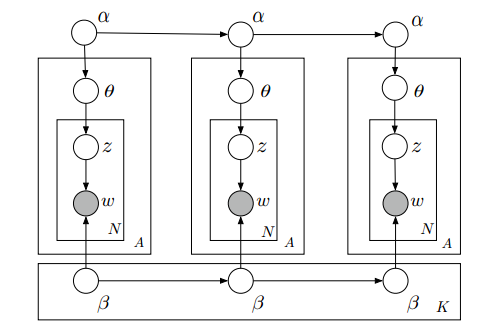
\includegraphics[width=0.7\textwidth]{dynamic_topic_model}
  \caption{Dynamic topic model. COPYRIGHT.}
  \label{fig:dtm}
\end{figure}
Effectively, Figure \ref{fig:dtm} is a sequential combination of the basic LDA model illustrated in Figure \ref{fig:lda}. In Figure \ref{fig:dtm}, one basic LDA model represents one time-slice. Also, the parameters $\alpha$ and $\beta$ are induced by their predecessors. More formal representation of the generative process is given in Algorithm 2 below. 
\begin{algorithm}[H]
\caption{Dynamic document generation.}
\label{alg:dynamic_document_generation}
\begin{algorithmic}[2]
\State $\beta_t | \beta_{t-1} \sim \mathcal{N}(\beta_{t-1}, \sigma^2I)$
\State $\alpha_t | \alpha_{t-1} \sim \mathcal{N}(\alpha_{t-1}, \delta^2I)$
\For {$d \leftarrow 1, M$}
\State $\eta_d \sim \mathcal{N}(\alpha_{t}, a^2I)$
\For {$n \leftarrow 1, N$}
\State $z_{d, n} \sim \mbox{Multinomial}(\pi(\eta_d))$
\State $w_{t, d, n} \sim \mbox{Multinomial}(\pi(\beta_t | z_{d, n}))$
\EndFor
\EndFor
\end{algorithmic}
\end{algorithm}

Algorithm 2 describe the generative process of the documents in time-slice $t$. The algorithm is initialised by drawing the parameters $\alpha_t$ and $\beta_t$ from the Gaussian distribution with the means given by the previous parameter values. Note that the parameters $\alpha_0$ and $\beta_0$ are the the special case. They can be initialised randomly, i.e. the mean of the Gaussian distribution is random. However, for the parameters $\alpha_0$ and $\beta_0$ we take larger variance values compared to $\alpha_t$ and $\beta_t$. The larger variance values  induce the initial time-slice with larger fluctuations in the topic and vocabulary term distributions; and the smaller variance values in the following time-slices induce the smoothness. Further, in lines 3--9, for every document in time-slice $t$ we execute the following procedure: for document $d$, we draw the topic distribution $\eta_d$ (the meaning of the parameter is equivalent to the previously introduced $\theta_d$); then, in lines 5--7, for every word in document $d$ we draw topic assignment $z_{d, n}$ and, finally, we draw word $w_{t, d, n}$. Note that the means for the Multinomial distributions are normalised by the use of \textit{parametrisation}. Parametrisation mapping $\pi$ is expressed as
\begin{equation}
\pi(x)_n = \dfrac{\exp{(x_n)}}{\sum^N_{i=1}\exp{(x_i)}}.
\end{equation}

% Inference
% Variational methods are a deterministic alternavive for stochastic simulation
% Two variations: Kalman filtering and wavelet regression
\par The authors have used variational methods to approximate the inference of the posterior. It is claimed that stochastic simulation (sampling-based variance methods) would be unable to scale with larger data sets. Further, the authors discuss two methods used for the variational inference: Kalman Filtering and Wavelet Regression. The implementation details of these methods can be found in the `Dynamic Topic Modelling' article \cite{blei_2006}. Note that the implementation details are provided in a brief manner suggesting the use of additional literature, these are also provided in the article. 

% Experiments
% - Evolution of Science
\par The dynamic topic model is evaluated by conducting an experiment on the journals of `Science'. The experiment is expected to infer the prevalent science fields and the prevalent vocabulary used in these fields. Note that the relevance of the science fields can be respectively obtained from the latent variables $\theta$ and $\phi$. That is, the authors would compare these variables throughout all time-slices in order to induce the reasoning over the prevalent science fields (by using $\theta$) and the prevalent vocabulary terms (by using $\phi$). The experiment has successfully established this notion of time-series. This is proved by comparing the inferred rises and falls of the scientific fields to the history of science. Note that the experiment has been performed both Kalman Filtering and Wavelet Regression methods. 

% Conclusion
\par By reviewing the original dynamic topic model, we have familiarised with the generative process which takes time-series into account. We have provided the visualisation of the model and introduced the algorithm for the generative process. Further, we have outlined the inference methods suggests be the authors. Finally, we have familiarised with the experiment settings which were used to infer time series in the articles of `Science'. 

%%%%%%%%%%%%%%%%%%%%%%%%%%%%%%%%%%%%%%%%%%%%%%%%%%%%%%%%%%%%%%%%%%%%%%%%%
%%%%%%%%%%%%%%%%%%%%%%%%%%%%%%%%%%%%%%%%%%%%%%%%%%%%%%%%%%%%%%%%%%%%%%%%%
%%%%%%%%%%%%%%%%%%%%%%%%%%%%%%%%%%%%%%%%%%%%%%%%%%%%%%%%%%%%%%%%%%%%%%%%%
\section{Proposed Approach}

% Section intro
% - Discussion over literature
% - Design of the model
% - Evaluation of the model
\par In this section, we will set up the approach of the project's execution. To start with, we will go over the literature reviewed in Section 3 to derive the promising techniques in terms of applicability to MSI data sets. Then, we will go over the high-level design and implementation requirements. Finally, we will set the basis for the model's evaluation. 

%%%%%%%%%%%%%%%%%%%%%%%%%%%%%%%%%%%%%%%%%%%%%%%%%%%%%%%%%%%%%%%%%%%%%%%%%
%%%%%%%%%%%%%%%%%%%%%%%%%%%%%%%%%%%%%%%%%%%%%%%%%%%%%%%%%%%%%%%%%%%%%%%%%

% Discussion over the literature
\subsection{Discussion}

% Intro
% - Literature review shows the mathematical underlying
% - Extract the relevant bits
\par Throughout the literature review, we have looked into the papers establishing the mathematical underlying of the LDA-like models. However, the approach in utilising those models in MSI like data sets have not been reviewed. Nevertheless, two sources of relevant research have been provided (the paper by Hooft et al. \cite{hooft} and the survey by Alonso et al. \cite{alonso-et-al}). Ultimately, this section is focused to emphasise the superior approaches of the previously reviewed papers; also, we will establish the appropriate techniques for the generative and inference processes.

% Generative processess
% - Comparison between static and dynamic data sets
\par The reviewed generative processes describe how the initial data is expected to be formed. Recall that we have reviewed two generative processes: static and dynamic. The static generative process is given by the initial LDA paper -- `Latent Dirichlet Allocation', and the dynamic generative processes is given by the `Dynamic Topic Models' paper. The applications of these generative processes are expressed respectively in Figure \ref{fig:static} and Figure \ref{fig:dynamic} below. 
\begin{figure}[H]
  \centering
  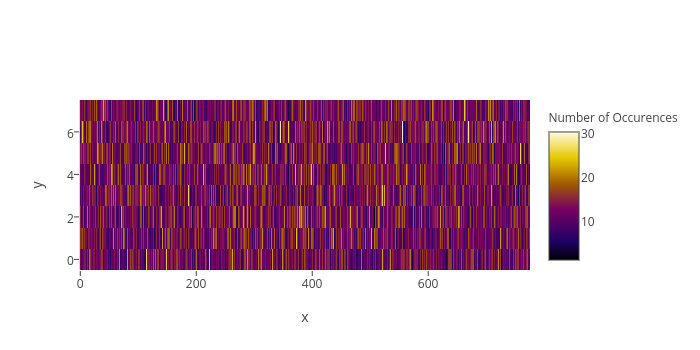
\includegraphics[width=0.7\textwidth]{static}
  \caption{Static generative process.}
  \label{fig:static}
\end{figure}
\begin{figure}[H]
  \centering
  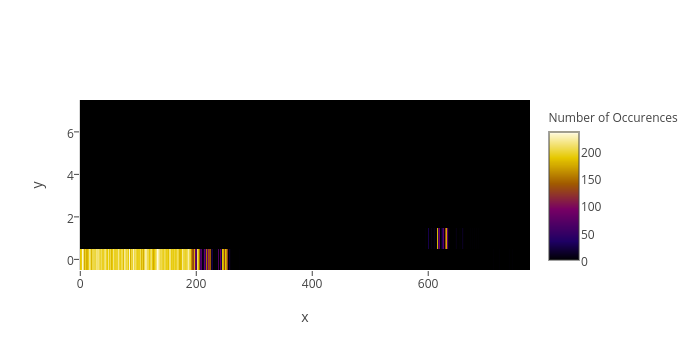
\includegraphics[width=0.7\textwidth]{dynamic}
  \caption{Dynamic generative process.}
  \label{fig:dynamic}
\end{figure}
In the previous plots, we have visualised the occurrences of a particular entity within a corpus. The static generative process suggests a random distribution of the entities, whereas the dynamic generative process induces a particular pattern. Since we expect the ions of same type be in clusters (rather than to be randomly distributed across the sample), the dynamic generative process is more appropriate to reflect the nature of the chemical entities patterns.  

% Generative process
% - Rather than sequential development, we induce a relationship between the documents

The initial dynamic topic modelling paper suggests to induce the time-series into the generative process of data sets. However, the way we capture the ions is done instantaneously for the whole corpus. Therefore, we are relaxing the assumption of time-series. Instead of that, we will use the dynamic topic modelling techniques to establish the relationship between the time-slices (even though we are not taking time into account, we will stick to the same terminology to preserve the consistency). For example, if we assume that the data is generated in a 1-dimensional manner, then time-slice $t$ would depends on its adjacent time-slices $t-1$ and $t+1$. However, since the image of the sample is 2-dimensional, there are more adjacent time-slices. This relationship is shown in Figure \ref{fig:2-d_generative_process} below.
\begin{figure}[H]
  \centering
  \includegraphics[width=0.5\textwidth]{2-d_generative_process}
  \caption{2-dimensional generative process.}
  \label{fig:2-d_generative_process}
\end{figure}
In the boundary case shown on the left, time-slice $t_{0,0}$ is related to three surrounding time-slices, whereas, in the general case indicated on the right side, time-slice $t_{1,1}$ relates to eight surrounding time-slices. Ultimately, the notion of dynamic topic modelling can be  preserved even upon relaxing the assumption of time-series.

% Inference
% - Stochastic and optimisation based methods
% - Evaluation
\par The reviewed inference techniques have covered the mathematical underlying of two approaches: stochastic (sampling-based) and optimisation (variational). The variational methods are discussed in the `Latent Dirichlet Allocation' and `Dynamic Topic Models' papers, and the sampling-based method is discussed in the `Finding Scientific Topics' paper. Since both methods have been utilised in the state-of-the-art topic modelling applications, we will implement both of them in order to set up a discussion for the developed model's evaluation. However, since the authors of `Dynamic Topic Models' has utilised only the variational methods, we have to address the compatibility of the sampling-based methods in terms of applicability to the dynamic topic modelling.


%%%%%%%%%%%%%%%%%%%%%%%%%%%%%%%%%%%%%%%%%%%%%%%%%%%%%%%%%%%%%%%%%%%%%%%%%
%%%%%%%%%%%%%%%%%%%%%%%%%%%%%%%%%%%%%%%%%%%%%%%%%%%%%%%%%%%%%%%%%%%%%%%%%
\subsection{Design}

% Intro
% - The required model supplements
\par By covering the design of the model, we will set up the requirements for the project's execution and propose methods which would supplement the techniques derived from the reviewed literature. To start with, we will address the dimensionality reduction of the MSI data sets. Then, we will introduce the additional data capturing requirements shifting the set-up of the generative process. Finally, we will suggest an approach for utilising sampling-based methodology in the dynamic topic modelling. 

% Dimensionality Reduction
% - Dictionary
% - Preprocessing
% -- Dismissing low intensity values
% -- Storing the ranges of ions
\par In order to address the scalability of the model in terms of the large MSI data sets, we will address two techniques for the dimensionality reduction: utilisation of a dictionary and pre-processing of the data. Both of these techniques reduce the sparsity of the data sets. To start with, the use of dictionary will eliminate the irrelevant use of memory by not storing the words which do not occur in the documents. For example, let's assume that the masses of the ions in our data can be represented as the set $\{1, 2, 3, 4, 5\}$, also assume that the ions can be represented in the form of a (mass, intensity) tuple. Then, if our sample contained two following documents: $\mathbf{w_0} = \{(1, 0.1), (2, 200), (3, 500)\}$ and $\mathbf{w_1} = \{(5, 300)\}$, the sample representation in matrix and dictionary forms would be interchangeable with the expressions given in Table \ref{tab:m_and_d} below.
\begin{table}[H]
\begin{center}
\begin{tabular}{|c||c|c|c|c|c|}
\hline
&1&2&3&4&5\\
\hline
$\mathbf{w_0}$&0.1&200&500&0&0\\
$\mathbf{w_1}$&0&0&0&0&300\\
\hline
\end{tabular}
\quad
\begin{tabular}{|c||c|c|c|c|c|}
\hline
&1&2&3&4&5\\
\hline
$\mathbf{w_0}$&0.1&200&500&$\O$&$\O$\\
$\mathbf{w_1}$&$\O$&$\O$&$\O$&$\O$&300\\
\hline
\end{tabular}
\end{center}
\caption{Matrix and dictionary representation of the data set.}
\label{tab:m_and_d}
\end{table}
Note that, in these settings, empty set symbol $\O$ represents a value which is not assigned to the memory; and the matrix and dictionary forms are respectively given on the left and right hand sides. It follows that the use of dictionary requires about as half as much memory. Another dimensionality reduction technique can be introduced by setting the minimum threshold value. That is, we can limit the data set by dismissing values which do not reach the sufficient significance criteria. If we set the threshold of intensity to be $1$, then the dictionary could be represented in Table \ref{tab:d_threshhold} below.
\begin{table}[H]
\begin{center}
\begin{tabular}{|c||c|c|c|c|c|}
\hline
&1&2&3&4&5\\
\hline
$\mathbf{w_0}$&\O&200&500&$\O$&$\O$\\
$\mathbf{w_1}$&$\O$&$\O$&$\O$&$\O$&300\\
\hline
\end{tabular}
\end{center}
\caption{The dictionary of the data set with the minimum intensity threshold of 1.}
\label{tab:d_threshhold}
\end{table}

% Ion grouping
\par As discussion in Section 1, the captured ions of same time are likely to have fluctuations in their masses. For this reason, we are applying another pre-processing step. By setting the threshold which indicated the maximum fluctuation between the masses of the ions, we would group the ions which are likely to represent the same type; also, we would reduce the dimensionality of the data set. By taking the example of the previous paragraph and setting the fluctuation tolerance to $1$, we obtain the data structure given in Table \ref{tab:d_f_threshhold} below.
\begin{table}[H]
\begin{center}
\begin{tabular}{|c||c|c|}
\hline
&[2,3]&[5,5]\\
\hline
$\mathbf{w_0}$&700&$\O$\\
$\mathbf{w_1}$&$\O$&300\\
\hline
\end{tabular}
\end{center}
\caption{The dictionary of the data set with the fluctuation threshold of 1.}
\label{tab:d_f_threshhold}
\end{table}
Notice that the masses are now represented by intervals, and the intensities below the threshold are summed together. Ultimately, by utilising the latter dimensionality reduction and ion grouping techniques, we establish data structure which would scale better compared to the initial data capturing settings.

% Generative process
% 3-D data sets
\par The generative process of the MSI data set discussed in the discussion over the reviewed literature has utilised 2-dimensional data set. However, we are expecting to work on 3-dimensional data sets. Therefore, the established relationship between time-slices is illustrated by Figure \ref{fig:3-d_generative_process} below.
\begin{figure}[H]
  \centering
  \includegraphics[width=0.7\textwidth]{3-d_generative_process}
  \caption{3-dimensional generative process.}
  \label{fig:3-d_generative_process}
\end{figure}
The time-slice indicated by the green colour, which is one of the boundary cases, is related to other elven time-slices indicated by the red colour. Note that in the general case, the time-slice would have twenty-six relating documents. Effectively, we have introduced the application settings of the dynamic topic modelling in the 3-dimensional space.  
% - To-ask: 4-dimensions (time-series)

% Inference
% - Metropolis--Hastings
\par In Section 3, we have addressed a sampling-based inference method -- Gibbs sampling. However, for the dynamic topic models, the latter method has to be reconsidered due to the change from Dirichlet to Gaussian distributions. Therefore, we will look into another MCMC based algorithm -- Metropolis--Hastings.
% - To-do: Analyse the details of the MH. 


%%%%%%%%%%%%%%%%%%%%%%%%%%%%%%%%%%%%%%%%%%%%%%%%%%%%%%%%%%%%%%%%%%%%%%%%%
%%%%%%%%%%%%%%%%%%%%%%%%%%%%%%%%%%%%%%%%%%%%%%%%%%%%%%%%%%%%%%%%%%%%%%%%%
\subsection{Evaluation}

% Intro
% - Spatial Smoothing
% - Two inference methods
% - Risk management
\par The developed technique addressing the spatial smoothing of the MSI data sets will evaluated by the model's performance. The performance will be assessed by investigating the inferred patterns of the captured ions. Also, we will utilise two different inference methods: sampling-based and variational. By having two model variations, we will be able to compare the time performance. Hence, we will be able to deduce which variation scales better with the size of the data sets. Finally, the section will be finished by investigating the possible risks. Also, we will provide a plan to mitigate these risks.  


% Evaluation/Experiments
\par

% Risks
\par 

% To-do:
% - Ask about experiments
% - Ask about risks
\par


%%%%%%%%%%%%%%%%%%%%%%%%%%%%%%%%%%%%%%%%%%%%%%%%%%%%%%%%%%%%%%%%%%%%%%%%%
%%%%%%%%%%%%%%%%%%%%%%%%%%%%%%%%%%%%%%%%%%%%%%%%%%%%%%%%%%%%%%%%%%%%%%%%%
%%%%%%%%%%%%%%%%%%%%%%%%%%%%%%%%%%%%%%%%%%%%%%%%%%%%%%%%%%%%%%%%%%%%%%%%%
\section{Work Plan}

% Intro
% - Tasks.
% - Schedule
% - Deliverables
\par In this section, we will outline the project milestones and deliverables. That is, we will outline the most important steps and provide the estimations in a form of Gantt chart. Further, the deliverables will be directly induced from the project's objectives and hypothesis (these are addressed in Section 2). The deliverables will contain both successful and successful outcomes of the set hypothesis.

\subsection{Schedule}

% Tasks
% - Design
% -- Investigate the literature on the spatial smoothing application in MSI data sets
% -- Design the dynamic topic model
% - Implementation
% -- Implement the generative process of the dynamic topic modelling with applied spatial smoothing
% -- Implement both sampling-based and variational inference to the dynamic topic model
% - Evaluation
% -- Test the performance of the applied spatial smoothing
% - Documentation/Presentation
% -- Dissertation
% -- Reports
% -- Presentation
\par The high-level plan of the project's execution include the following milestones: design, implementation, evaluation, and documentation/presentation. To establish a basis for the design, we will continuously review the literature on spatial smoothing, MSI, and dynamic topic models. Then, the implementation will require the utilisation of spatial smoothing in the generative process of the dynamic topic model; also, for the inference, we will implement both: sampling-based and variational methods. Further, the evaluation will be conducted by assessing the performance of the developed models. Finally, the results will be documented in a form of weekly reports, dissertation, and presentation.

% Dates
% - Non-continuous
% - Estimations
\par The outlined tasks will not be necessarily executed in sequential manner. For some of the tasks, we will use parallel approach as given in Figure \ref{fig:gantt} below.

\begin{figure}[H]
\begin{ganttchart}[
hgrid, 
vgrid,
y unit chart=.8cm
]{1}{15}

\gantttitle{Weeks}{15} \\
\gantttitlelist{1,...,15}{1} \\

\ganttgroup{Design}{1}{7} \\
\ganttbar{Dynamic Generative Process}{1}{5} \\
\ganttbar{Spatial Smoothing}{3}{7} \ganttnewline

\ganttgroup{Implementation}{3}{10} \\
\ganttbar{Dynamic Generative Process}{3}{6} \\
\ganttbar{Inference Methods}{4}{7} \\
\ganttbar{Spatial Smoothing}{7}{10} \\

\ganttgroup{Evaluation}{8}{11} \\
\ganttbar{Usability}{8}{10} \\
\ganttbar{Performance}{9}{11} \ganttnewline

\ganttgroup{Documentation/Presentation}{2}{15} \\
\ganttbar{Reports}{2}{11} \\
\ganttbar{Dissertation}{10}{15} \ganttnewline
\ganttbar[
=TBA
]{Presentation}{12}{14}

\end{ganttchart}
\caption{Gantt chart of the project's execution.}
\label{fig:gantt}
\end{figure}



% Code
% Dissertation
\subsection{Deliverables}

% Conclusion
\par 

%%%%%%%%%%%%%%%%%%%%%%%%%%%%%%%%%%%%%%%%%%%%%%%%%%%%%%%%%%%%%%%%%%%

\bibliography{mprop}
\bibliographystyle{plain}
% To-do: list, in alphabetical order by author and date
\end{document}
